\documentclass{article}

%\usepackage[utf8]{inputenc}		% LuaTex do not need this
%\usepackage[T1]{fontenc}			% LuaTex do not need this
\usepackage{fontspec}				% LuaTex need this
\usepackage{lmodern}
\usepackage{comment}
\usepackage[a4paper]{geometry}
\usepackage{graphicx}
	\graphicspath{ {Bilder/} }

%%%%%%%%%%%%%%%%%%%%%%%%%%%%%%%%%%%%%%%%%%%%%%%%%%%%%%%%%%%%%%%%%%%%%%%%%%%%%%%%
%
% https://tex.stackexchange.com/questions/82993/how-to-change-the-name-of-document-elements-like-figure-contents-bibliogr
% https://tex.stackexchange.com/questions/186946/changing-the-autoref-name-for-chapter
%
%\usepackage[ngerman]{babel}		% LuaTex do not need this
\usepackage{polyglossia}
	\setdefaultlanguage[spelling=new]{german}
	\addto\captionsgerman{
		\renewcommand{\figurename}{Abbildung}
		\renewcommand{\figureautorefname}{Abbildung}
		\renewcommand{\equationautorefname}{Gleichung}
	}


%%%%%%%%%%%%%%%%%%%%%%%%%%%%%%%%%%%%%%%%%%%%%%%%%%%%%%%%%%%%%%%%%%%%%%%%%%%%%%%%
%
% LATEX Mathematical Symbols
% https://reu.dimacs.rutgers.edu/Symbols.pdf
% https://en.wikibooks.org/wiki/LaTeX/Mathematics
%
\usepackage{amssymb}
\usepackage{amsthm}

%%%%%%%%%%%%%%%%%%%%%%%%%%%%%%%%%%%%%%%%%%%%%%%%%%%%%%%%%%%%%%%%%%%%%%%%%%%%%%%%
%
% algorithm2e.sty — package for algorithms
% http://ctan.mirrors.hoobly.com/macros/latex/contrib/algorithm2e/doc/algorithm2e.pdf
%
\usepackage[
	ngerman,
	linesnumbered,
	boxed,
%	algochapter,
%	rightnl,
%	figure,
]{algorithm2e}
	% Then you can adjust the spacing between the body of the algorithm and its
	% caption through the command \SetAlCapSkip.
	\SetAlCapSkip{1em}
	% Restyling the caption in an algorithm created with algorithm2e
	% https://tex.stackexchange.com/questions/112294/restyling-the-caption-in-an-algorithm-created-with-algorithm2e/112295
	\SetAlgoCaptionSeparator{:}
	\renewcommand\AlCapFnt{\normalfont}
	% Algorithm2e modify line numbers
	% https://tex.stackexchange.com/questions/100145/algorithm2e-modify-line-numbers
	\SetNlSty{textbf}{}{:}
	% Sets the value of the space between the line numbers and the text, by default 1em.
	\SetNlSkip{2em}
	%\SetAlgoRefName{QXY}

%%%%%%%%%%%%%%%%%%%%%%%%%%%%%%%%%%%%%%%%%%%%%%%%%%%%%%%%%%%%%%%%%%%%%%%%%%%%%%%%
%
% TikZ
%
\usepackage{tikz}
	\usetikzlibrary{
		arrows,
		petri,
		topaths,
		graphs,
		graphdrawing,
		graphs.standard,
		shapes}
	\usegdlibrary{trees, layered}
\usepackage{tkz-berge}
\usepackage{tkz-graph}
\makeatletter
\pgfmathdeclarefunction{alpha}{1}{%
	\pgfmathint@{#1}%
	\edef\pgfmathresult{\pgffor@alpha{\pgfmathresult}}%
}
%%%%%%%%%%%%%%%%%%%%%%%%%%%%%%%%%%%%%%%%%%%%%%%%%%%%%%%%%%%%%%%%%%%%%%%%%%%%%%%%
%
% https://www.dante.de/events/Archiv/dante2012/Programm/Vortraege/vortrag-ferber.pdf
%
\usepackage[
	breaklinks,
	colorlinks,
	linkcolor=black,
	urlcolor=black,
	citecolor=black,
	pdfencoding=auto,
]{hyperref}
%%%%%%%%%%%%%%%%%%%%%%%%%%%%%%%%%%%%%%%%%%%%%%%%%%%%%%%%%%%%%%%%%%%%%%%%%%%%%%%%
%
% bibtex vs. biber and biblatex vs. natbib
%	- https://tex.stackexchange.com/questions/25701/bibtex-vs-biber-and-biblatex-vs-natbib
% The biblatex Package - Programmable Bibliographies and Citations
% 	- http://ftp.math.purdue.edu/mirrors/ctan.org/macros/latex/exptl/biblatex/doc/biblatex.pdf
% Biblatex citation order
%	- https://tex.stackexchange.com/questions/51434/biblatex-citation-order
% 		- sorting=ydnt: Sort by year (descending), name, title.
%		- sorting=none: Do not sort at all. All entries are processed in citation order.
%
\usepackage[backend=biber,style=numeric-comp,sorting=none]{biblatex}
	\addbibresource{Quellen.bib}
%%%%%%%%%%%%%%%%%%%%%%%%%%%%%%%%%%%%%%%%%%%%%%%%%%%%%%%%%%%%%%%%%%%%%%%%%%%%%%%%
%
%
%
\usepackage{verbatim}
%\usepackage[vario]{fancyref}
\usepackage{float}
\usepackage{subcaption}
	\captionsetup{subrefformat=parens}


%%%%%%%%%%%%%%%%%%%%%%%%%%%%%%%%%%%%%%%%%%%%%%%%%%%%%%%%%%%%%%%%%%%%%%%%%%%%%%%%
%
%
%
\title{Hamiltonsche Graphen und das\\ Traveling Salesman Problem (TSP)}

\author{
  Albert Kasdorf\and
  Andreas Janster\and
  Alex Bibanaev\and
  Georg Braun}
\date{09.05.2018}

% https://en.wikibooks.org/wiki/LaTeX/Theorems
\newtheorem{mydef}{Definition}
\newtheorem{mylem}{Lemma}
\newtheorem{mysat}{Satz}


%%%%%%%%%%%%%%%%%%%%%%%%%%%%%%%%%%%%%%%%%%%%%%%%%%%%%%%%%%%%%%%%%%%%%%%%%%%%%%%%
%
%
%
\begin{document}
\tikzstyle{vertex}=[circle,fill=black!25,minimum size=15pt,inner sep=0pt]
\tikzstyle{selected vertex} = [vertex, fill=red!24]
\tikzstyle{edge} = [draw,thick,-]
\tikzstyle{weight} = [font=\small]
\tikzstyle{selected edge} = [draw,line width=5pt,-,red!50]
\tikzstyle{ignored edge} = [draw,line width=5pt,-,black!20]
\pgfdeclarelayer{background}
\pgfsetlayers{background,main}

\maketitle


%%%%%%%%%%%%%%%%%%%%%%%%%%%%%%%%%%%%%%%%%%%%%%%%%%%%%%%%%%%%%%%%%%%%%%%%%%%%%%%%
%
%
%
%\section{Definition (Nur temporär; Entfernen in endgültiger Version)}
%
%\begin{mydef}
%	Einfacher Graph/Simple Graph: Ein einfacher Graph besitzt weder Schleifen noch parallele Kanten.
%\end{mydef}
%
%\begin{mydef}
%	Zusammenhängender Graph: Von zwischen jedem Knoten u, v gibt es einen Weg.
%\end{mydef}
%
%\begin{mydef}
%	Vollständiger Graph: Jeder Knoten eines Graphens ist benachbart.
%\end{mydef}
%
%\begin{mydef}
%	Weg: Ein Kantenzug heißt Weg, wenn alle Kanten verschieden sind.
%\end{mydef}
%
%\begin{mydef}
%	Einfacher Weg: Ein Weg heißt einfach, wenn kein Knoten doppelt durchlaufen wird.
%\end{mydef}
%
%\begin{mydef}
%	Kreis: Ein Kreis ist ein Weg mit gleichem Anfangs- und Endknoten.
%\end{mydef}
%
%\begin{mydef}
%	Einfacher Kreis: Ein einfacher Kreis ist ein Kreis, in dem außer den Endknoten kein Knoten doppelt durchlaufen wird.
%\end{mydef}
%
%\begin{mydef}
%	Eine Euler-Tour in einem Graphen G = (V,E) ist ein Weg, der jede Kante e E genau einmal enthält und dessen Anfangs- und Endknoten identisch sind.
%\end{mydef}
%
%\begin{mydef}
%	Satz: Ein zusammenhängender Graph besitzt genau dann eine Euler-Tour, wenn alle Knoten des Graphen geraden Grad haben.
%\end{mydef}
%
%\begin{mydef}
%	Ein Hamiltonkreis in einem Graphen ist ein Kreis, der alle Knoten genau einmal enthält.
%\end{mydef}

%\begin{mydef}\label{definition_hamilton_graph}
%	Ein Graph heißt hamiltonsch oder Hamilton-Graph, wenn in ihm ein Kreis existiert, der jeden Knoten genau einmal enthält. Ein solcher Kreis heißt auch Hamilton-Kreis.
%\end{mydef}


%%%%%%%%%%%%%%%%%%%%%%%%%%%%%%%%%%%%%%%%%%%%%%%%%%%%%%%%%%%%%%%%%%%%%%%%%%%%%%%%
%
%
%
\section{Hamiltonsche Graphen}


%%%%%%%%%%%%%%%%%%%%%%%%%%%%%%%%%%%%%%%%%%%%%%%%%%%%%%%%%%%%%%%%%%%%%%%%%%%%%%%%
%
%
%
\subsection{Motivation}

Das junge Pärchen Anna und Bernd planen ihre Hochzeit. Der Großteil der Aufgaben ist bereits geplant und erledigt. Nur über den Sitzplan für das Hochzeitsessen grübeln beide schon des längeren und kommen zu keinem Ergebnis. Ihr Wunsch ist es, dass während des Essens eine ausgelassen Stimmung herrscht. Daher soll neben jedem Gast, jeweils zu seiner linken und rechten Seite, zwei ihm bekannte Person sitzen.

Eines Abend als Bernd sich mit seinen alten Studienkollegen trifft kommt ihm die zündende Idee. Das Sitzplatz-Problem ließe sich mit einem Graphen modellieren. Die Gäste werden durch Knoten beschrieben und die Bekanntschaft zwischen zwei Gästen durch eine Kante, siehe \autoref{fig:acquaintance_graph_a}. Wenn es einen Kreis in dem Graphen gibt, in dem jeder Knoten genau einmal vorkommt, wäre das Sitzplatz-Problem gelöst. Nach einigen Versuchen hat er einen Kreis gefunden, der alle Knoten miteinander verbindet, siehe \autoref{fig:acquaintance_graph_b}.

\begin{figure}[h]
	\centering
	\subcaptionbox{\label{fig:acquaintance_graph_a}}[.49\linewidth]
	{
		%\begin{tikzpicture}[scale=0.45, every node/.style={transform shape}]
		\begin{tikzpicture}[scale=0.45]
		\node (A) at (-1,+0) [circle, draw, ultra thick] {A};
		\node (B) at (+1,+0) [circle, draw, ultra thick] {B};
		\node (C) at (-4,+0) [circle, draw] {C};
		\node (D) at (-4,-3) [circle, draw] {D};
		\node (E) at (-4,+4) [circle, draw] {E};
		\node (F) at (-6,+2) [circle, draw] {F};
		\node (G) at (+0,+2) [circle, draw] {G};
		\node (H) at (+4,+4) [circle, draw] {H};
		\node (I) at (+4,+0) [circle, draw] {I};
		\node (J) at (+2,-3) [circle, draw] {J};
		
		\draw (A)--(B) (A)--(C) (A)--(D) (A)--(E) (A)--(F) (A)--(G);
		\draw (B)--(D) (B)--(I) (B)--(J) (B)--(G) (B)--(H);
		\draw (C)--(D) (C)--(F);
		\draw (D)--(F);
		\draw (E)--(F) (E)--(G) (E)--(H);
		\draw (F)--(G);
		\draw (G)--(H) (G)--(I);
		\draw (I)--(J);
		\end{tikzpicture}
	}
	\subcaptionbox{\label{fig:acquaintance_graph_b}}[.49\linewidth]
	{
		%\begin{tikzpicture}[scale=0.45, every node/.style={transform shape}]
		\begin{tikzpicture}[scale=0.45]
		\node (A) at (-1,+0) [circle, draw, ultra thick] {A};
		\node (B) at (+1,+0) [circle, draw, ultra thick] {B};
		\node (C) at (-4,+0) [circle, draw] {C};
		\node (D) at (-4,-3) [circle, draw] {D};
		\node (E) at (-4,+4) [circle, draw] {E};
		\node (F) at (-6,+2) [circle, draw] {F};
		\node (G) at (+0,+2) [circle, draw] {G};
		\node (H) at (+4,+4) [circle, draw] {H};
		\node (I) at (+4,+0) [circle, draw] {I};
		\node (J) at (+2,-3) [circle, draw] {J};
		
		\draw (A)--(B) (A)--(C) (A)--(D) (A)--(E) (A)--(F) (A)--(G);
		\draw (B)--(D) (B)--(I) (B)--(J) (B)--(G) (B)--(H);
		\draw (C)--(D) (C)--(F);
		\draw (D)--(F);
		\draw (E)--(F) (E)--(G) (E)--(H);
		\draw (F)--(G);
		\draw (G)--(H) (G)--(I);
		\draw (I)--(J);
		
		\draw[black, ultra thick] (A)--(B)--(J)--(I)--(G)--(H)--(E)--(F)--(C)--(D)--(A);
		\end{tikzpicture}
	}
	\caption{Links: Ein Graph der die Bekanntschaft zwischen den Hochzeitsgästen modelliert. Rechts: Ein Kreis in dem Bekanntschaftsgraphen der jeden Gast zwei im bekannte Gäste zuweist.}
	\label{fig:acquaintance_graph}
\end{figure}


%%%%%%%%%%%%%%%%%%%%%%%%%%%%%%%%%%%%%%%%%%%%%%%%%%%%%%%%%%%%%%%%%%%%%%%%%%%%%%%%
%
%
%
%\subsection{Icosian-Spiel}

% Such paths and cycles are named after Hamilton (1856), who described, in a letter to his friend Graves, a mathematical game on the dodecahedron (figure 4 . 2 ~ ) in which one person sticks five pins in any five consecutive vertices and the other is required to complete the path so formed to a spanning cycle. A graph is hamiltonian if it contains a Hamilton cycle. The dodecahedron is hamiltonian (see figure 4 . 2 ~ ~ the) ; Herschel graph (figure 4.2b) is nonhamiltonian, because it is bipartite and has an odd number of vertices.


%%%%%%%%%%%%%%%%%%%%%%%%%%%%%%%%%%%%%%%%%%%%%%%%%%%%%%%%%%%%%%%%%%%%%%%%%%%%%%%%
%
%
%
\subsection{Definition}

Wie es bereits aus dem einleitenden Beispiel zu erkennen ist, wird in einem Graphen ein Kreis gesucht, der alle Knoten so miteinander verbindet, dass außer dem Start- und Endknoten kein Knoten doppelt vorkommt. Ein Graph mit diesen Eigenschaften wird wie folgt definiert:
% Ein Graph der diese Eigenschaft erfüllt heißt hamiltonsch oder Hamilton-Graph und der Kreis dementsprechend Hamilton-Kreis.

\begin{mydef}\label{thm:definition_hamilton_graph}
	Ein Graph heißt hamiltonsch oder Hamilton-Graph, wenn in ihm ein Kreis existiert, der jeden Knoten genau einmal enthält. Ein solcher Kreis heißt auch Hamilton-Kreis.\cite{busing2010graphen}
\end{mydef}

Die Hamilton-Eigenschaft ähnelt der Euler-Eigenschaft, nur das bei dem ersten alle Knoten genau einmal durchlaufen werden und beim zweiten alle Kanten. Ein Graph kann dabei beide, eine oder keine der beiden Eigenschaft in sich vereinen, siehe \autoref{fig:combination_of_euler_and_hamilton}.

\begin{figure}[h]
	\centering
	\subcaptionbox{\label{fig:combination_of_euler_and_hamilton_a}}[.24\linewidth]
	{
		\begin{tikzpicture}[scale=0.75]
			\node (A) at (0,0) [circle, draw] {A};
			\node (B) at (0,2) [circle, draw] {B};
			\node (C) at (1,3) [circle, draw] {C};
			\node (D) at (2,2) [circle, draw] {D};
			\node (E) at (2,0) [circle, draw] {E};
			\node (F) at (1,1) [circle, draw] {F};
			\draw (A)--(B)--(C)--(D)--(E)--(F)--(A);
		\end{tikzpicture}
	}
	\subcaptionbox{\label{fig:combination_of_euler_and_hamilton_b}}[.24\linewidth]
	{
		\begin{tikzpicture}[scale=0.75]
		\node (A) at (0,0) [circle, draw] {A};
		\node (B) at (0,2) [circle, draw] {B};
		\node (C) at (1,3) [circle, draw] {C};
		\node (D) at (2,2) [circle, draw] {D};
		\node (E) at (2,0) [circle, draw] {E};
		\node (F) at (1,1) [circle, draw] {F};
		\draw (A)--(B) (A)--(F) (A)--(E);
		\draw (B)--(C) (B)--(D) (B)--(F);
		\draw (D)--(C) (D)--(F) (D)--(E);
		\draw (E)--(F);
		\end{tikzpicture}
	}
	\subcaptionbox{\label{fig:combination_of_euler_and_hamilton_c}}[.24\linewidth]
	{
		\begin{tikzpicture}[scale=0.75]
		\node (A) at (0,0) [circle, draw] {A};
		\node (B) at (0,2) [circle, draw] {B};
		\node (C) at (1,3) [circle, draw] {C};
		\node (D) at (2,2) [circle, draw] {D};
		\node (E) at (2,0) [circle, draw] {E};
		\node (F) at (1,1) [circle, draw] {F};
		\draw (A)--(F) (A)--(E);
		\draw (B)--(C) (B)--(F);
		\draw (D)--(C) (D)--(F);
		\draw (E)--(F);
		\end{tikzpicture}
	}
	\subcaptionbox{\label{fig:combination_of_euler_and_hamilton_d}}[.24\linewidth]
	{
		\begin{tikzpicture}[scale=0.75]
		\node (A) at (0,0) [circle, draw] {A};
		\node (B) at (0,2) [circle, draw] {B};
		\node (C) at (1,3) [circle, draw] {C};
		\node (D) at (2,2) [circle, draw] {D};
		\node (E) at (2,0) [circle, draw] {E};
		\node (F) at (1,1) [circle, draw] {F};
		\draw (F)--(A) (F)--(B) (F)--(C) (F)--(D) (F)--(E);
		\end{tikzpicture}
	}
	\caption{Der Graph \subref{fig:combination_of_euler_and_hamilton_a} ist sowohl eulersch als auch hamiltonsch, \subref{fig:combination_of_euler_and_hamilton_b} ist nur hamiltonsch, \subref{fig:combination_of_euler_and_hamilton_c} ist nur eulersch und \subref{fig:combination_of_euler_and_hamilton_d} ist weder noch.}
	\label{fig:combination_of_euler_and_hamilton}
\end{figure}

Ähnlich wie mit den Euler-Graphen werden in den folgenden zwei Abschnitten einige Kriterien untersucht, um herauszufinden ob ein Graph einen Hamilton-Kreis besitzt oder nicht. Um es gleich vorweg zu nehmen, bisher konnte kein allgemein gültiges Kriterium gefunden werden, das die Existenz eines Hamilton-Kreises in polynomieller Laufzeit bestätigt.

%%%%%%%%%%%%
%
% Knotengrad
%
%%%%%%%%%%%%
\subsection{Knotengrad}

\begin{mylem}\label{thm:lemma_degree_of_one}
	Ein hamiltonscher Graph enthält keinen Knoten mit Grad 1.
\end{mylem}

Bei dem Lemma~\autoref{thm:lemma_degree_of_one} handelt es sich um das einfaches Ausschlusskriterium für die Existenz eines Hamilton-Kreises. Befindet sich in dem Graphen ein Knoten mit einem Grad von eins, dann ist es nicht mehr möglich von diesem Knoten aus einen weiteren zu besuchen und somit kann auch der Kreis nicht geschlossen werden, siehe \autoref{fig:graph_with_min_degree_of_one}.

\begin{figure}[h]
	\centering
	\begin{tikzpicture}
		\node (A) at (0,0) [circle, draw] {A};
		\node (B) at (0,2) [circle, draw] {B};
		\node (C) at (1,1) [circle, draw] {C};
		\node (D) at (2,1) [circle, draw] {D};
		\draw (A)--(B)--(C)--(D);
		\draw (A)--(C);
	\end{tikzpicture}
	\caption{Ein Graph mit einem Minimalgrad von eins kann keinen Hamilton-Kreis enthalten.}
	\label{fig:graph_with_min_degree_of_one}
\end{figure}

Im Jahre 1952 hat der britischer Physiker Dirac ein Kriterium aufgestellt mit der die Existenz eines Hamilton-Kreises in einem Graphen nachgewiesen werden kann, siehe Satz~\autoref{thm:satz_dirac}.

% Was sagt dieser Satz aus? Wenn man viele Kanten hat, dann ist es wahrscheinlicher einen hamilton kreis zu finden.
\begin{mysat}\label{thm:satz_dirac}
	Sei G ein einfacher Graph mit mindestens drei Knoten, für den außerdem $\delta(G)\geq 0.5\cdot n$ gilt. Dann enthält der Graph einen Hamilton-Kreis.
\end{mysat}

Die Kernaussage ist dabei, das jeder Knoten des Graphen eine gewisse Mindestanzahl an Kanten zu benachbarten Knoten besitzen soll. Hier durch werden, zum einem isolierte Knoten und zum anderen Bäume ausgeschlossen.

Es sei zu erwähnen, dass der Satz von Dirac eine hinreichende jedoch keine notwendige Bedingung für die Existenz eines Hamilton-Kreises ist. Es gibt Graphen die das Kriterium von Dirac nicht erfüllen und trotzdem einen Hamilton-Kreis besitzen, siehe \autoref{fig:hamilton_without_dirac}.

\begin{figure}[h]
	\centering
	\begin{tikzpicture}
	\node (A) at (0,0) [circle, draw] {A};
	\node (B) at (0,1) [circle, draw] {B};
	\node (C) at (1,2) [circle, draw] {C};
	\node (D) at (2,1) [circle, draw] {D};
	\node (E) at (2,0) [circle, draw] {E};
	\draw (A)--(B)--(C)--(D)--(E)--(A);
	\end{tikzpicture}
	\caption{Ein Graph der einen Hamilton-Kreis enthält, jedoch das Kriterium von Dirac nicht erfüllt.}
	\label{fig:hamilton_without_dirac}
\end{figure}


%%%%%%%%%%%%%%
% Zusammenhang
%%%%%%%%%%%%%%
\subsection{Zusammenhang}

\begin{mylem}
	Falls ein Graph hamiltonsch ist, dann ist er auch zusammenhängend.
\end{mylem}

Wenn es einen Hamilton-Kreis in einem Graphen gibt, dann hat jeder Knoten mindestens zwei adjazente Knoten. Somit sind sowohl isolierte Knoten als auch nicht zusammenhängende Teilgraphen ausgeschlossen. Die Rückrichtung gilt jedoch nicht, ein Baum ist zwar zusammenhängend, aber nicht hamiltonsch.

% Zusammenhang, klappt nicht beim Petersen-Graph
\begin{mysat}\label{thm:decay_to_connected_components}
	Für jeden hamiltonschen Graphen gilt: Wenn k Knoten aus dem Graphen gelöscht werden, zerfällt der Graph in höchstens k Zusammenhangskomponenten.
\end{mysat}

Den Satz~\autoref{thm:decay_to_connected_components} kann man sich dabei sehr vereinfacht wie folgt vorstellen. Man nehme einen Faden und verbinde diesen zu einem Kreis. Wenn der Faden jetzt an einer Stelle zerschnitten wird, entsteht maximal ein Fadenstück. Mit jedem weiteren Schnitt zerfällt ein Fadenstück zu maximal zwei weiteren Fadenstücken, es können niemals mehr Fadenstücke entstehen als Schnitte getätigt wurden. Zerfällt hingegen der Graph in mehr Zusammenhangskomponenten als Schnitte getätigt wurden, so kann in dem Graphen kein Hamilton-Kreis existiert haben, siehe \autoref{fig:one_cut_two_connected_components}.

\begin{figure}[h]
	\centering
	\subcaptionbox{}[.49\linewidth]
	{
		\begin{tikzpicture}[scale=1.]
		\node (A) at (0,0) [circle, draw] {A};
		\node (B) at (0,2) [circle, draw] {B};
		\node (C) at (2,1) [circle, draw] {C};
		\node (D) at (4,0) [circle, draw] {D};
		\node (E) at (4,2) [circle, draw] {E};
		\draw (C)--(A) (C)--(B) (C)--(D) (C)--(E);
		\draw (A)--(B) (D)--(E);
		\end{tikzpicture}
	}
	\subcaptionbox{}[.49\linewidth]
	{
		\begin{tikzpicture}[scale=1.]
		\node (A) at (0,0) [circle, draw] {A};
		\node (B) at (0,2) [circle, draw] {B};
		\node (C) at (2,1) [circle, draw, dashed] {C};
		\node (D) at (4,0) [circle, draw] {D};
		\node (E) at (4,2) [circle, draw] {E};
		\draw[dashed] (C)--(A) (C)--(B) (C)--(D) (C)--(E);
		\draw (A)--(B) (D)--(E);
		\end{tikzpicture}
	}
	\caption{Durch das herauslösen des Knoten C entstehen zwei Zusammenhangskomponenten. Ein Hamilton-Kreis kann in diesem Graphen nicht vorhanden sein.}
	\label{fig:one_cut_two_connected_components}
\end{figure}

An dem Petersen-Graph kann man gut erkennen, das es bei dem Satz~\autoref{thm:decay_to_connected_components} um ein reines Ausschlusskriterium handelt. Den der Petersen-Graph erfüllt zwar die Bedingung, dass nie mehr Komponenten entstehen, als Knoten aus dem Graphen herausgelöst werden, jedoch enthält er keinen Hamilton-Kreis, siehe \autoref{fig:petersen_graph}.

\begin{figure}[h]
	\centering
	\begin{tikzpicture}[every node/.style={draw,circle}]
	\graph [clockwise,math nodes] {
		subgraph C_n [V={a,b,c,d,e}, name=A, radius=2cm];
		subgraph I_n [V={f,g,h,i,j}, name=B, radius=1cm];
		\foreach \x [evaluate={%
			\i=alpha(\x);
			\j=alpha(mod(\x+1,5)+6);
			\k=alpha(\x+5);}] in {1,...,5}{
			A \i -- B \k;
			B \j -- B \k;
		}
	};
	\end{tikzpicture}
	\caption{Der Petersen-Graph enthält keinen Hamilton-Kreis.}
	\label{fig:petersen_graph}
\end{figure}


%%%%%%%%%%%%%%%%%%%%%%%%%%%%%%%%%%%%%%%%%%%%%%%%%%%%%%%%%%%%%%%%%%%%%%%%%%%%%%%%
%
%
%
\section{Traveling Salesman Problem}

Das Traveling-Salesman-Problem (TSP) (dt. Problem des Handlungsreisenden) ist ein kombinatorisches Optimierungsproblem. Die Herausforderung besteht, darin eine optimale Reihenfolge für den Besuch einer vorgegebenen Menge von Orten so zu wählen, dass die zurückgelegte Strecke des Handlungsreisenden möglichst kostenminimal und die erste Station gleich der letzten Station ist.

\begin{mydef}
	Travelling-Sales-Problem: Gegeben sei ein vollständiger Graph K\textsubscript{n} mit positiven Gewichten \textit{c(e)} auf den einzelnen Kanten  \textit{e}. Gesucht ist ein Hamilton-Kreis \textit{C} in K\textsubscript{n} mit minimalem Gewicht c(C), wobei gilt
	\[c(C) =  \sum_{e \in C}  c(e) \]
\end{mydef}

\subsection{Modellierung als Graph}

In der Praxis kann dieses Problem in verschiedenen Planungssituationen auftreten. Den die Begriffe „Ort“ und „Strecke“ können auf verschiedene Anwendungsbereiche abstrahiert werden. Damit mathematische Verfahren zur Lösung verwendet werden können, muss eine reale Situation zunächst durch ein einfaches Modell abgebildet werden. Orte können nicht nur durch Städte, sondern zum Beispiel auch durch Kunden oder Bohrlöcher repräsentiert werden, während die Entfernung für Zeiten, Grade oder Kosten stehen kann. Solche Problemszenarien können zudem durch Zusatzbedingungen wie Zeitfenster oder eingeschränkte Ressourcen erweitert werden. Das Problem des Handlungsreisenden ist ein NP-vollständiges Problem.

\subsubsection*{Asymmetrisches und symmetrisches TSP}

Gerichtete Graphen eignen sich zur Modellierung von allgemeinen asymmetrischen TSP, weil hier können die Kanten in Hin- und Rückrichtung unterschiedliche Gewichte haben. Beim symmetrischen TSP gilt für alle Knotenpaare, das die Kantenlängen in beide Richtungen identisch sind, somit eignen sich ungerichteten Graphen zur Darstellung.

\subsection{Lösungsmethoden}

Grundsätzlich gibt es zwei verschiedene Kategorien von Lösungsansätzen: \textit{exakte Algorithmen} und \textit{Heuristiken}. Die Lösung von \textit{exakten Algorithmen} ist optimal und muss zusätzlich durch einen Beweis gezeigt werden. \textit{Heuristiken} versuchen innerhalb eines Zeitrahmens eine zulässige Lösung, die recht nah an der Optimallösung ist, zu finden.

\begin{figure}[H]
	\centering
	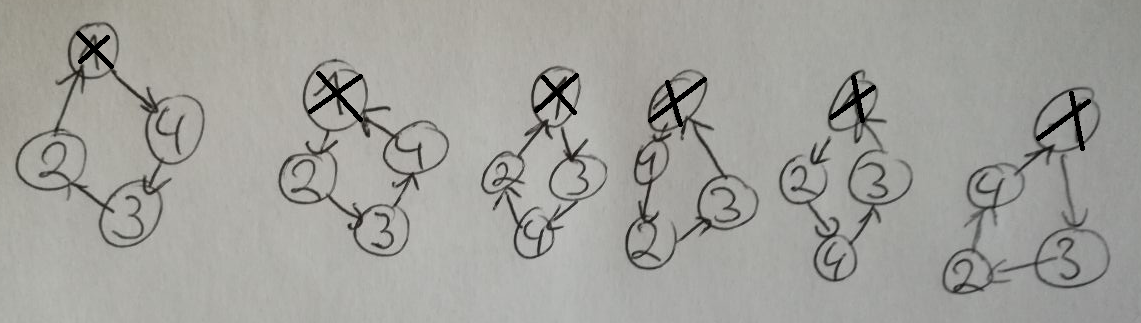
\includegraphics[width=1\textwidth]{Graphen.png}
	\caption{Alle Lösungen für eine Paketauslieferung an drei Häuser (PLATZHALTER BILD)}
	\label{fig:Rundreise}
\end{figure}

Um einen \textit{exakten Algorithmus} zu beleuchten, stellen wir zunächst ein triviales Beispiel für eine Planungssituation auf, und modellieren dieses mithilfe der Graphentheorie. In diesem Szenario haben wir ein Paketdienst, der drei Pakete an drei verschiedene Häuser ausliefern muss. Dazu brauchen wir vier Knoten, wobei ein Knoten unseren Startfiliale darstellt und die drei weiteren die Zielhäuser, wohin die Pakte geliefert werden müssen. Das Ziel ist es eine Tour (Hamilton-Kreis) zu definieren.
\par Um die Lösung zu finden, erzeugen wir einen Hamilton-Kreis nach der anderen und merken uns jene. Anschließend bestimmen wir die Länge jedes Hamilton-Kreises. Um die beste Tour zu finden, wählen wir den kürzesten Hamilton-Kreis aus. Die \autoref{fig:Rundreise} zeigt alle zulässigen Touren für unser Szenario.

\begin{description}
	\item[F:] Wie viele verschiedene Touren gibt es in einem vollständigen Graphen mit n Knoten? Zeigen Sie das der Satz~\autoref{thm:count_of_hamilton_circle_in_asm_graph} gilt.
\end{description}

\begin{mysat}\label{thm:count_of_hamilton_circle_in_asm_graph}
	Ein vollständiger asymmetrischer Graph enthält genau $(n-1)!$ Hamilton-Kreise.
\end{mysat}

Beim symmetrischen TSP wird nicht zwischen einer Tour und ihrer Rückrichtung unterschieden. Für die Lösungen in \autoref{fig:Rundreise} würde es bedeuten, dass die Lösungen \textit{(b)} \textit{(d)} und \textit{(f)} wegfallen. Somit gilt:

\begin{mysat}
	Ein vollständiger symmetrischer Graph enthält genau $0.5 * (n-1)!$ Hamilton-Kreise.
\end{mysat}

Für unser Beispiel mit drei Zielen konnten wir leicht eine optimale Lösung finden. Doch was würde es bedeuten, wenn die Anzahl der Ziele auf 21 steigen würde? Die Fakultätsfunktion steigt rasant, die Konsequenz wir müssen $0.5 * 21! = 2.554.547.108.585.472.0000$ Lösungen generieren und im Anschluss daran die Kosten berechnen.

Für praxisrelevante Szenarien bedeutet es eine unvermeidbare Laufzeitexplosion. Solange $P = NP$ gilt, wird es kein beweisbar schnelles Verfahren zur optimalen Lösung des TSP geben. Das ist die Ursache dafür, dass in der Praxis Heuristiken verwendet werden, aber auch weil man oft gar nicht an der Optimallösung interessiert ist. Aufgrund der Tatsache, dass die verwendeten Daten schon Fehler enthalten oder nicht genau ermittelt werden können. Eine Städtetour durch Europa mit einem Fahrzeug ist von vielen Faktoren abhängig wie: Fahrzeugtyp, Wetter, Verkehr. In diesem Beispiel wäre die Forderung nach Optimalität ein Overkill.


\subsection{Das Bohren von Leiterplatten}

Das bisherige Wissen kann ebenfalls auf andere Gebiete abgebildet werden. Beispielsweise das Herstellen einer elektronischen Leiterplatine zählt dazu. Dabei geht es darum, dass möglichst schnell \textit{n} Löcher in eine Platine gebohrt werden müssen. Je schneller eine Platine fertig ist, desto mehr können produziert werden. Das Bohren eines einzelnen Lochs ist ohne Qualitätsverlust nicht zu beschleunigen. Um jedoch Zeit zu sparen, darf der Bohrer keine unnötigen Wege zurücklegen. Die meisten Fräs- oder Bohrmaschinen in der Leiterplattenindustrie sind nur mit zwei Motoren bzw. Schienen ausgestattet um die gesamte Platine zu erreichen. Deshalb kann man sich das System als \textit{2D-Koordinatensystem} vorstellen. Der eine Motor steuert den Bohrer auf der X-Achse, also die rechts-links-Bewegung. Der andere fährt den Bohrer entlang der Y-Achse bzw. nach vorne oder hinten. Damit nur die minimale Wegstrecke zurückgelegt wird, also keine Zeit verschwendet wird, muss der optimale Zyklus für den Bohrer errechnet werden.

Zu aller erst muss klar sein, wie der Abstand zwischen zwei Bohrlöchern bestimmt werden kann. Wenn man bedenkt, dass der Bohrer sich über Loch A befindet und zu Loch C kommen möchte, wird schnell klar, dass der eine Stellmotor seine Bewegung schneller beendet hat, als der andere und deshalb eine Ruhephase hat bzw. auf den zweiten Stellmotor warten muss, siehe  \autoref{abb_leiterplatine}).

\begin{figure}[H]
	\centering
	%  \subfigure{}
	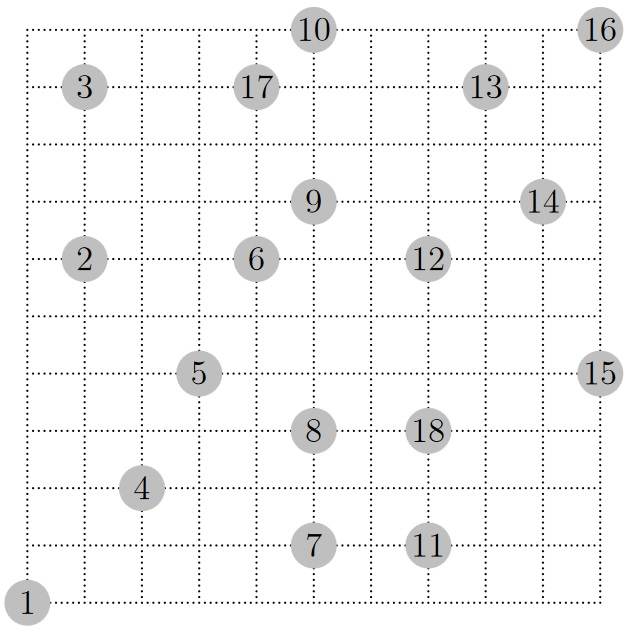
\includegraphics[width=0.6\textwidth]{leiterplatine.jpg}
	\caption{Beispielbohrungen einer Leiterplatine}
	\label{abb_leiterplatine}
\end{figure}

Es reicht also nicht den einfachen Abstand zwischen den beiden Punkten auszumessen oder auszurechnen (euklidischer Abstand, vgl. Pythagoras). Das würde nur funktionieren wenn die Motoren sich diagonal fortbewegen. Der maximale Abstand muss ausgerechnet und genutzt werden:
\[d\textsubscript{max} = max\{ |x\textsubscript{2} - x\textsubscript{1}| , |y\textsubscript{2} - y\textsubscript{1}|\} \]
In \autoref{abb_leiterplatine2} sind beispielhaft die Kantengewichte der Kante A-C in Sekunden sowie die Bewegung der zwei Stellmotoren zu sehen. Während Stellmotor auf der X-Achse lediglich eine Sekunde benötigt um den Bohrer auf die korrekte Position zu manövrieren, benötigt der Stellmotor auf der Y-Achse 4 Sekunden. Das Gewicht der Kante ist also mit \textit{4} zu bemessen.

\begin{figure}[H]
	\centering
	%  \subfigure{}
	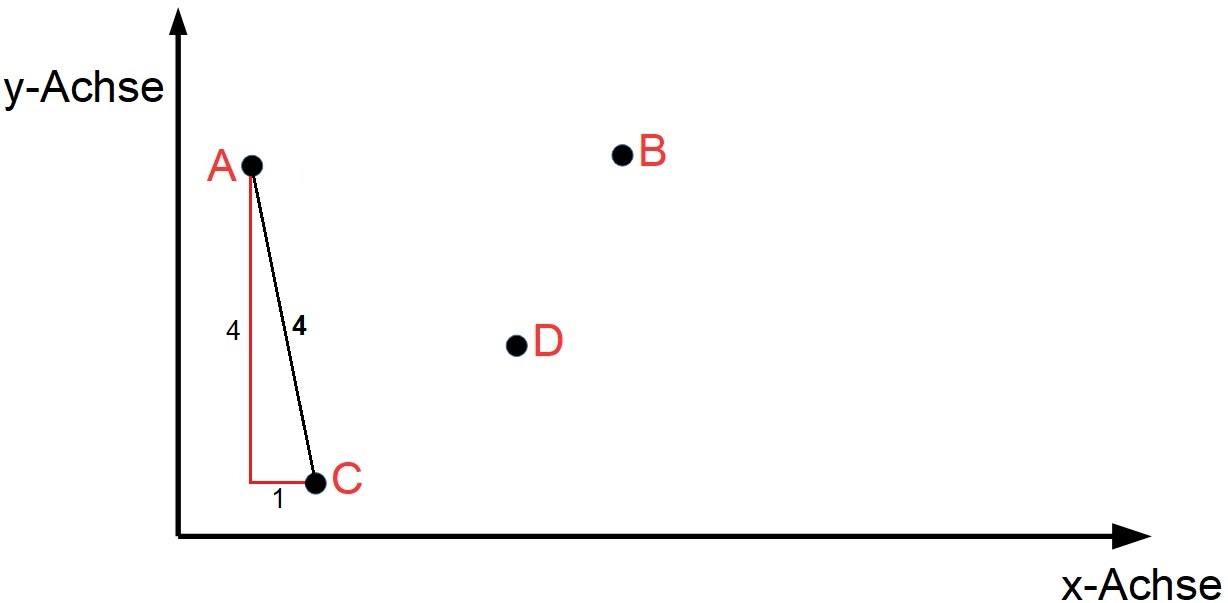
\includegraphics[width=0.6\textwidth]{leiterplatine2.jpg}
	\caption{Bohrerbewegung zwischen Loch A und Loch C}
	\label{abb_leiterplatine2}
\end{figure}

Bedenkt man nun, das man eine zeit optimierte Rundreise für den Bohrer finden möchte, bildet man aus dem Graphen einen vollständigen Graphen. Es sollen also jeder Knoten mit allen anderen verbunden sein. In dem Beispiel geht man davon aus, dass der Bohrer sich durch das ganze Feld ohne Hindernisse bewegen kann. Nur so kann sichergestellt sein, dass das Hinzufügen von neuen Kanten im Graphen zu keinen Problemen führt.
\\
\begin{description}
	\item[F:] Wie könnte eine möglichst gute Rundreise auf der Leiterplatte Aussehen?
\end{description}




%%%%%%%%%%%%%%%%%%%%%%%%%%%%%%%%%%%%%%%%%%%%%%%%%%%%%%%%%%%%%%%%%%%%%%%%%%%%%%%%
%
%
%
\section{Algorithmen}

\subsection{Nearest-Neighbor-Heuristik}

Die Nearest-Neighbor Heuristik ist ein heuristisches Verfahren, welches genutzt wird um eine Lösung für das Problem des Handlungsreisenden zu ermitteln. Es handelt sich dabei um einen Greedy-Algorithmus der wie folgt funktioniert:

\begin{algorithm}
\KwIn{Ein vollständiger Graph $T$ mit Kantengewichten $c(e)$}
\KwOut{Ein Hamilton-Kreis}
\SetKwInOut{Parameter}{Schritt 1:}
\Parameter{Wähle einen beliebigen Knoten als Startknoten $v$ }
\SetKwInOut{Parameter}{Schritt 2:}
\Parameter{Ermittle die niedrigste Kante welche den aktuellen Knoten $v$ mit einem unbesuchten Knoten $v_u$ verbindet.}
\SetKwInOut{Parameter}{Schritt 3:}
\Parameter{Setze $v = v_u$ }
\SetKwInOut{Parameter}{Schritt 4:}
\Parameter{Wenn noch nicht alle Knoten besucht wurden gehe wieder zu Schritt 2.}
\SetKwInOut{Parameter}{Schritt 5:}
\Parameter{Füge die Kante vom letzten besuchten Knoten zum Startknoten hinzu um den Kreis zu schließen.}
\caption{Nearest-Neighbor Algorithmus}
\end{algorithm}

Eine beispielhafte Anwendung des Algorithmus wird anhand einer Routenfindung zwischen den Städten Aachen (AC), Bonn (BN), Düsseldorf (D), Frankfurt (F), Köln (K) und Wuppertal (W) demonstriert. Angenommen die Entfernungen entsprechen den Angaben in der Tabelle in Abbildung \ref{fig:nearest-neighbor-beispiel}

%% Start

\begin{figure}[h]
	\centering
	\subcaptionbox{\label{tbl:entfernungen-staedte}}[.49\linewidth]
	{
		\begin{tabular}{ |c|c|c|c|c|c|c| }
\hline
 & AC & BN & D& F & K & W \\ 
\hline
AC &  & 91 & 80 & 259 & 70 & 121 \\ 
\hline
BN & 91 &  & 77 & 175 & 27 & 84 \\ 
\hline
D & 80 & 77 &  & 232 & 47 & 29 \\ 
\hline
F & 259 & 175 & 232 &  & 189 & 236 \\ 
\hline
K & 70 & 27 & 47 & 189 &  & 55 \\ 
\hline
W & 121 & 84 & 29 & 236 & 55 &  \\ 
\hline
\end{tabular}
	}
	\subcaptionbox{\label{fig:nearest-neighbor-tour}}[.49\linewidth]
	{
\begin{tikzpicture}[scale=0.8, auto,swap]
    % First we draw the vertices
    \foreach \pos/\name in {{(-4,-1)/AC}, {(1,-2)/BN}, {(-0.75,2)/D},
                            {(5,-5)/F}, {(-0.5,0)/K}, {(1,2.25)/W}}
        \node[vertex] (\name) at \pos {$\name$};
    % Connect vertices with edges and draw weights	
\draw [edge, ->] (AC) to node[]{1.} (K);
\draw [edge, ->] (K) to node[]{2.} (BN);
\draw [edge, ->] (BN) to node[]{3.} (D);
\draw [edge, ->] (D) to node[]{4.} (W);
\draw [edge, ->] (W) to node[]{5.} (F);
\draw [edge, ->] (F) to node[]{6.} (AC);
\end{tikzpicture}
	}
\caption{Links: Entfernung der Städte in km. Rechts: Tour des Nearest-Neighbor Algorithmus.}
\label{fig:nearest-neighbor-beispiel}
\end{figure}

%% Ende


Mit Aachen als Startpunkt würde der Algorithmus die Tour in \autoref{fig:nearest-neighbor-beispiel} konstruieren und ein Ergebnis mit 698 Kilometern liefern. Es wird auch deutlich, dass diese Lösung nicht das beste Ergebnis ist. Tatsächlich lässt sich ein relativ simples Beispiel konstruieren welches zeigt, dass die Nearest Neighbor Heuristik auch eine beliebig schlechte Lösung für das Problem des Handlungsreisenden liefern kann. In \autoref{fig:nearest-neighbor-beispiel} (a) ist dieser Graph mit den jeweiligen Kantengewichten dargestellt. Wählt man den Knoten $1$ als Startknoten und fordert, dass $x>1$ ist, so liefert der Nearest-Neighbor Algorithmus den Hamilton-Kreis in \autoref{fig:nearest-neighbor-beispiel} (b) als Ergebnis. Das Ergebnis enthält eine Kante mit variablen Kantengewicht. Die Kosten betragen also $1+1+1+x = x +3$. Aufgrund der Variable kann das Ergebnis des Algorithmus beliebig schlecht sein. Ein weiterer Hamilton-Kreis ist in \autoref{fig:nearest-neighbor-beispiel} (c) dargestellt. In diesem Kreis betragen die Kosten $1+2+1+2 = 6$.
Falls  $x>3$ gilt handelt es dabei um einen optimalen Kreis. 

% Start
\begin{figure}[h]
	\centering
	\subcaptionbox{\label{fig:nearest-neighbor-graph}}[.32\linewidth]
	{
		\begin{tikzpicture}[scale=0.8, auto,swap]
    % First we draw the vertices
    \foreach \pos/\name in {{(-2,1)/1}, {(2,1)/2}, {(-2,-1)/3},{(2,-1)/4}}
        \node[vertex] (\name) at \pos {$\name$};
\node at (0,1.25) {1};
\node at (2.25,0) {1};
\node at (-2.25,0) {$x$};
\node at (0,-1.25) {1};
\node at (-1.2,0.3) {2};
\node at (1.2,0.3) {2};
% Nearest Neighbor
\draw [edge] (1) to (2);
\draw [edge] (2) to (4);
\draw [edge] (4) to (3);
\draw [edge] (3) to (1);	
\draw [edge](1) to (4);
\draw [edge](2) to (3);
\end{tikzpicture}
	}
	\subcaptionbox{\label{fig:nearest-neighbor-ergebnis}}[.32\linewidth]
	{
\begin{tikzpicture}[scale=0.8, auto,swap]
    % First we draw the vertices
    \foreach \pos/\name in {{(-2,1)/1}, {(2,1)/2}, {(-2,-1)/3},{(2,-1)/4}}
        \node[vertex] (\name) at \pos {$\name$};
\node at (0,1.25) {1};
\node at (2.25,0) {1};
\node at (-2.25,0) {$x$};
\node at (0,-1.25) {1};
% Nearest Neighbor
\draw [edge] (1) to (2);
\draw [edge] (2) to (4);
\draw [edge] (4) to (3);
\draw [edge] (3) to (1);	
\end{tikzpicture}
	}
	\subcaptionbox{\label{fig:nearest-neighbor-optimum}}[.32\linewidth]
	{
\begin{tikzpicture}[scale=0.8, auto,swap]
    % First we draw the vertices
    \foreach \pos/\name in {{(-2,1)/1}, {(2,1)/2}, {(-2,-1)/3},{(2,-1)/4}}
        \node[vertex] (\name) at \pos {$\name$};
\node at (0,1.25) {1};
\node at (0,-1.25) {1};
\node at (-1.2,0.3) {2};
\node at (1.2,0.3) {2};
% Nearest Neighbor
\draw [edge](1) to (4);
\draw [edge](2) to (3);
\draw [edge](1) to (2);
\draw [edge](4) to (3);
\end{tikzpicture}
	}
\caption{Links: Beispiel Graph. Mitte: Ergebnis Nearest-Neighbor. Rechts: Optimale Lösung falls $x>3$}
\label{fig:nearest-neighbor-beispiel}
\end{figure}
% Ende





\subsection{Doppelter-Baum-Algorithmus}
\subsubsection{Funktionsweise}
Der Doppelte-Baum Algorithmus von Rosenkranz, Stearns und Lewis aus dem Jahr 1977 berechnet einen Hamilton-Kreis. Zunächst wird der Algorithmus formal beschrieben und anschließend anhand eines Beispiels illustriert. 

Der Algorithmus sieht wie folgt aus:

\begin{algorithm}
\KwIn{Ein vollständiger Graph $K_n$ mit Kantengewichten $ c(e) $}
\KwOut{Ein Hamilton-Kreis}
\SetKwInOut{Parameter}{Schritt 1:}
\Parameter{Konstruiere einen minimal spannenden Baum $T$ von $K_n$.}
\SetKwInOut{Parameter}{Schritt 2:}
\Parameter{Verdopple alle Kanten von $T$ (daraus resultiert ein eulerscher Graph $T_d$).}
\SetKwInOut{Parameter}{Schritt 3:}
\Parameter{Berechne eine Euler-Tour in $T_d$.}
\SetKwInOut{Parameter}{Schritt 4:}
\Parameter{Durchlaufe die Euler Tour von einem Startknoten aus. Falls dabei ein Knoten schon besucht wurde, nehme die Abkürzung zum nächsten unbesuchten Knoten auf der Tour.}
\caption{Doppelter-Baum-Algorithmus}
\end{algorithm}

Um ein besseres Verständnis für den Algorithmus zu bekommen wird dieser anhand eines Beispielgraphen erläutert. Der vollständige Graph für den ein Hamilton-Kreis gefunden werden soll ist in \autoref{fig:ursprungs-graf-blank} dargestellt. Der Algorithmus fordert als Eingabe einen vollständigen Graphen mit Kantengewichten. Als Kantengewichte wird der euklidische Abstand zwischen den jeweiligen Knoten genutzt. Für eine übersichtlichere Darstellung wurde in der Abbildung auf die Einzeichnung der Kantengewichte verzichtet.

\begin{figure}[H]
\centering
\begin{tikzpicture}[scale=0.8]
    % Draw a 7,11 network
    % First we draw the vertices
    \foreach \pos/\name in {{(0,0)/a}, {(0,-2)/b},  {(1,-4)/c},
                            {(-3,-1.5)/d}, {(-5,-3)/e}, {(-4,0.5)/f}, {(3,1.25)/g}, {(3,-1)/h}}
        \node[vertex] (\name) at \pos {$\name$}; 
    \foreach \source/ \dest /\weight in {a/b/0, a/c/0, a/d/0, a/e/0, a/f/0, a/h/0, a/g/0, b/c/0, b/d/0, b/e/0, b/f/0, b/g/0, c/d/0, c/f/0, c/h/0, c/g/0, c/e/0, d/h/0, d/g/0, d/e/0, d/f/0, e/f/0, e/g/0, e/h/0, f/h/0, f/g/0, b/h/0, h/g/0}
        \path[edge] (\source) -- node[weight] {} (\dest);  
\end{tikzpicture}
\caption{Vollständiger Beispielgraph (Kantengewichte nicht eingezeichnet)}
\label{fig:ursprungs-graf-blank}
\end{figure}

Der erste Schritt des Algorithmus erfordert die Konstruktion eines minimal spannenden Baumes $T$. Dieser ist in \autoref{fig:ursprungs-graf-mst} dargestellt.

\begin{figure}[H]
\centering
\begin{tikzpicture}[scale=0.8, auto,swap]
    % Draw a 7,11 network
    % First we draw the vertices
    \foreach \pos/\name in {{(0,0)/a}, {(0,-2)/b},  {(1,-4)/c},
                            {(-3,-1.5)/d}, {(-5,-3)/e}, {(-4,0.5)/f}, {(3,1.25)/g}, {(3,-1)/h}}
        \node[vertex] (\name) at \pos {$\name$};
    % Connect vertices with edges and draw weights
    \foreach \source/ \dest /\weight in {b/a/0, c/b/0, b/d/0, d/e/0, d/f/0, b/h/0, h/g/0}
        \path[edge] (\source) -- node[weight] {} (\dest);
\end{tikzpicture}
\caption{Minimal spannender Baum}
\label{fig:ursprungs-graf-mst}
\end{figure}

Im zweiten Schritt werden die Kanten aus dem minimal spannenden Baum $T$ verdoppelt, sodass ein eulerscher Graph $T_d$ entsteht. In diesem Graph wird wie im nächsten Schritt gefordert eine Euler-Tour konstruiert. In \autoref{fig:ursprungs-graf-eulertour} ist ein Beispiel für eine Euler Tour eingezeichnet.

\begin{figure}[H]
\centering
\begin{tikzpicture}[scale=0.8, auto,swap]
    % Draw a 7,11 network
    % First we draw the vertices
    \foreach \pos/\name in {{(0,0)/a}, {(0,-2)/b},  {(1,-4)/c},
                            {(-3,-1.5)/d}, {(-5,-3)/e}, {(-4,0.5)/f}, {(3,1.25)/g}, {(3,-1)/h}}
        \node[vertex] (\name) at \pos {$\name$};
    % Connect vertices with edges and draw weights	
\draw [edge, bend angle=-20, bend left, ->] (c) to node[]{1} (b);		
\draw [edge, bend angle=-20, bend left, ->] (b) to node[]{2} (a);			
\draw [edge, bend angle=-20, bend left, ->] (a) to node[]{3} (b);			
\draw [edge, bend angle=-20, bend left, ->] (b) to node[]{4} (d);			
\draw [edge, bend angle=-20, bend left, ->] (d) to node[]{5} (e);			
\draw [edge, bend angle=-20, bend left, ->] (e) to node[]{6} (d);			
\draw [edge, bend angle=-20, bend left, ->] (d) to node[]{7} (f);			
\draw [edge, bend angle=-20, bend left, ->] (f) to node[]{8} (d);		
\draw [edge, bend angle=-20, bend left, ->] (d) to node[]{9} (b);			
\draw [edge, bend angle=-20, bend left, ->] (b) to node[]{10} (h);			
\draw [edge, bend angle=-20, bend left, ->] (h) to node[]{11} (g);			
\draw [edge, bend angle=-20, bend left, ->] (g) to node[]{12} (h);			
\draw [edge, bend angle=-20, bend left, ->] (h) to node[]{13} (b);	
\draw [edge, bend angle=-20, bend left, ->] (b) to node[]{14} (c);	
\end{tikzpicture}
\caption{Euler-Tour}
\label{fig:ursprungs-graf-eulertour}
\end{figure}

Anhand der dargestellten Euler-Tour wird nun die Vorgehensweise des vierten Schritts im Algorithmus erläutert. In diesem Schritt wird der Hamilton-Kreis ermittelt. Als Startpunkt wird der Knoten $c$ gewählt. Der resultierende Kreis ist in \autoref{fig:ursprungs-graf-hamiltonkreis} dargestellt. Von $c$ beginnend foglt man der Euler-Tour zu $b$. Von dort aus geht es weiter zu $a$. Bei einem Versuch der Euler-Tour weiter zu folgen stellt man fest, dass diese zum bereits besuchten Knoten $b$ führt. Der nächste unbesuchte Knoten in der Euler-Tour ist der Knoten $d$. Um dort hin zu kommen wird die Kante von $a$ zu $d$ gewählt (Erinnerung: Es handelt sich um einen vollständigen Graphen. Deshalb ist es möglich die direkte Verbindung zu nutzen). Von dort aus wird wieder der Euler-Tour zu $e$ gefolgt. Auch dort ist die Verfolgung der Euler-Tour zu $d$ nicht mehr möglich, da dieser Knoten bereits besucht wurde. Der nächste unbesuchte Knoten auf der Tour ist $f$. Wie auch zuvor wird nun die direkte Kante von $e$ nach $f$ genutzt. Bei dem Versuch der Euler-Tour wieder zu folgen bemerkt man, dass der nächste Knoten $d$ auch schon besucht wurde. Der darauf folgende Knoten $b$ wurde auch schon besucht. Erst der darauf folgende Knoten $h$ wurde noch nicht besucht, sodass die Kante von $f$ nach $h$ genutzt wird. Nach dem vorgestellten Schema wird weiter verfahren bis letztendlich alle Knoten besucht wurden. Die zum Erreichen der Knoten genutzten Kanten bilden somit den resultierenden Hamilton-Kreis.

\begin{figure}[H]
\centering
\begin{tikzpicture}[scale=0.8, auto,swap]
    % Draw a 7,11 network
    % First we draw the vertices
    \foreach \pos/\name in {{(0,0)/a}, {(0,-2)/b},  {(1,-4)/c},
                            {(-3,-1.5)/d}, {(-5,-3)/e}, {(-4,0.5)/f}, {(3,1.25)/g}, {(3,-1)/h}}
        \node[vertex] (\name) at \pos {$\name$};
    % Connect vertices with edges and draw weights	
\draw [edge, ->] (c) to node[]{} (b);
\draw [edge, ->] (b) to node[]{} (a);
\draw [edge, ->] (a) to node[]{} (d);
\draw [edge, ->] (d) to node[]{} (e);
\draw [edge, ->] (e) to node[]{} (f);
\draw [edge, ->] (f) to node[]{} (h);
\draw [edge, ->] (h) to node[]{} (g);
\draw [edge, ->] (g) to node[]{} (c);
\end{tikzpicture}
\caption{Hamilton-Kreis}
\label{fig:ursprungs-graf-hamiltonkreis}
\end{figure}

\subsubsection{Dreiecksungleichung}
Mit den Kosten $c$ zweier Knoten bezeichnet man das Kantengewicht der  Kante, welche diese Knoten verbindet.
\begin{mydef}\label{thm:definition_dreiecksungleichung}
Die Dreiecksungleichung garantiert bei einem vollständigen Graphen, dass für alle Knoten $u$,$v$ und $w$ gilt:

\begin{equation}
c(u,v) \leq c(u,w) + c(w,v)
\end{equation}

\end{mydef}

Im Kern sagt dies aus, dass der direkte Weg von einem Knoten u nach v kürzer ist, als der Umweg über einen zusätzlichen Knoten w, siehe \autoref{fig:dreiecksungleichung}.

\begin{figure}[H]
\centering
\begin{tikzpicture}[scale=0.8, auto,swap]
    % Draw a 7,11 network
    % First we draw the vertices
    \foreach \pos/\name in {{(0,0)/u}, {(4,0)/v}, {(2,2)/w}}
        \node[vertex] (\name) at \pos {$\name$};
    % Connect vertices with edges and draw weights
    \foreach \source/ \dest /\weight in {u/v/0, u/w/0, w/v/0}
        \path[edge] (\source) -- node[weight] {} (\dest);
\end{tikzpicture}
\caption{Dreiecksungleichung}
\label{fig:dreiecksungleichung}
\end{figure}



\subsubsection{Abschätzung des Doppelten-Baum-Algorithmus}
Der Doppelter-Baum-Algorithmus liefert zwar einen Hamilton-Kreis, jedoch ist dieser nicht zwangsläufig optimal. Erweitert man die Eingabe Vorschrift des Algorithmus dahingehend, dass die Dreiecksungleichung erfüllt ist, so lässt sich das Ergebnis zumindest eingrenzen. Eine obere Schranke wird wie folgt festgelegt. Die durch den Algorithmus bestimmte Tour ist maximal doppelt so lang wie eine optimale Tour. Formal lässt es sich wie folgt ausdrücken:

\begin{mysat}\label{thm:doppelterbaum-obere-grenze}
$K_n$ sei ein vollständiger Graph mit Kantengewichten welche die Dreiecksungleichung erfüllen. Ferner sei $T'$ das Ergebnis des Doppelten-Baum-Algorithmus und $OPT$ eine optimale Lösung. Dann gilt
\begin{equation}
c(T') \leq 2 * c(OPT).
\label{eq:test}
\end{equation}
\end{mysat}

% Beweis
Dieser Satz lässt sich wie folgt beweisen. Die Tour $T'$ kann maximal doppelt so lang sein wie die Kosten des minimalen Spannbaums $T$.

\begin{equation}
c(T') \leq 2 * c(T)
\end{equation}

Die Begründung dafür ist, dass im Algorithmus der minimal-spannende Baum verdoppelt wird und somit die Euler-Tour mit der Länge $2 * c(T)$ entsteht. Bei der Berechnung der Hamilton-Tour wird die Euler-Tour verfolgt. Ist dabei auf dem Weg zum nächsten Knoten ein bereits besuchter Knoten vorhanden, so wird der direkte Weg zu diesem genommen (siehe Algorithmus Schritt 4). Aufgrund der Dreiecksungleichung ist der direkte Weg kürzer als der zuvor geplante Umweg über den schon bereits besuchten Knoten. Somit wurde eine obere Schranke für das Ergebnis des Algorithmus aufgezeigt. Eine untere Schranke lässt sich durch folgende Annahme finden: Entfernt man eine Kante aus der optimalen Tour $OPT$, resultiert das in einem spannenden Baum. Dieser ist nicht billiger als der minimal-spannende Baum $T$. Es gilt also:

\begin{equation}
c(T) \leq c(OPT)
\end{equation}

Die Kombination aus der oberen und unteren Schranke führt zu folgendem Ergebnis was wiederum der obigen \autoref{eq:test} entspricht.

\begin{equation}
c(T') \leq 2 * c(T) \leq 2 * c(OPT)
\end{equation}



%%%%%%%%%%%%%%%%%%%%%%%%%%%%%%%%%%%%%%%%%%%%%%%%%%%%%%%%%%%%%%%%%%%%%%%%%%%%%%%%
%
% Literatur
%
% 	- http://linorg.usp.br/CTAN/macros/latex/contrib/biblatex/doc/biblatex.pdf
% 		- bibnumbered, bibintoc
%	- https://de.sharelatex.com/learn/Bibliography_management_with_biblatex
%
\nocite{busing2010graphen}
\nocite{jungnickel1994graphen}
\printbibliography[heading=bibnumbered,title={Literatur}]


\end{document}
